% !TeX encoding = UTF-8
% !TeX spellcheck = fr_FR
% !TeX root = ../mythesis.tex
% !TeX program = pdflatex (build)
%%% TeXmaker : no 'magic comments' but set Root with Options > Set as master file
\graphicspath{{./}{./fig/}{./chap_stimulated_hawking/fig/}}

\chapter{Experimental observation of stimulated Hawking radiation in a polariton quantum fluid}
\label{chap:stimulated_hawking}



In the previous chapter, we demonstrated the experimental realization of a transcritical flow in a polariton quantum fluid through precise optical pump shaping. This allowed us to engineer the fluid's density and velocity profiles to form a transcritical region, a key ingredient for the emergence of a sonic horizon. Additionally, we presented experimental evidence of negative-energy modes in this region, confirming the necessary conditions for the observation of the Hawking effect.

Building on these achievements, this chapter focuses on the experimental observation of stimulated Hawking radiation in a polariton fluid. Stimulated emission provides a controlled way to probe the Hawking effect by injecting a coherent state into the upstream region and measuring its scattering into outgoing modes. This approach allows us to directly study the amplification of positive-energy modes and the role of negative-energy modes in the transcritical region.
The experimental realization of stimulated Hawking radiation involves several key steps. First, we describe the setup used to inject coherent states into the polariton fluid and the techniques employed to measure the outgoing modes. 
Next, we detail the partial reconstruction of the scattering matrix, which encodes the mixing of positive- and negative-energy modes and provides direct evidence of energy amplification.
 Finally, we present the results of these measurements, discuss the agreement with theoretical predictions and the robustness of the stimulated Hawking effect.
The results presented in this chapter not only validate the theoretical predictions of stimulated emission but also establish a pathway toward the observation of spontaneous Hawking radiation. By leveraging the unique properties of polariton fluids, this work demonstrates the potential of these systems as a platform for exploring fundamental aspects of quantum field theory in curved spacetime and beyond.





\section{Interferometric measurement of the scattering matrix }
\label{sec:principle_measurement}

We aim at solving the scattering problem of a coherent state injected in the upstream region impinging on the horizon. Doing so, it is possible
to partially reconstruct the scattering matrix. This approach is complementary of what has already been done in other works in which 
the stimulating field was coming from the transcritical region. ???????? 

\subsection{Challenges of the measurement}

\begin{figure}
    \centering
    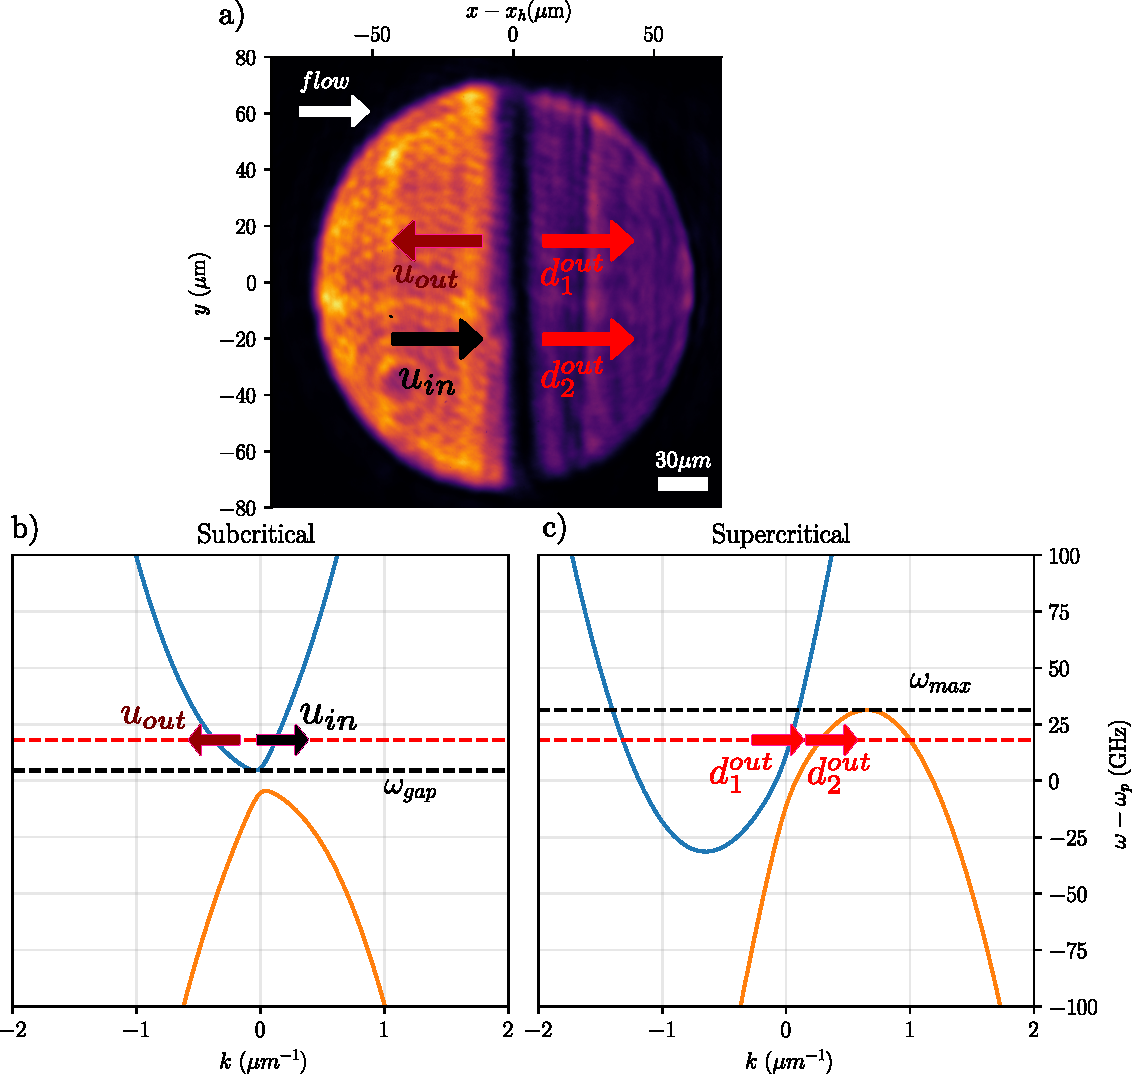
\includegraphics[width=1\textwidth]{chap_stimulated_hawking/fig/typical_dens_2D.pdf}
    \caption{\textbf{a)} Real space image of a transcritical flow of polaritons with detuning $\delta(0)=29 GHz$ and wavevectors $k_u=0.2 \mu m^{-1}$ and $k_d=0.6\mu m^{-1}$. The black arrow represents the impinging mode $u_{in}$ while the blue arrows represent the outgoing modes $u_{out}$, $d_1^{out}$ and $d_2^{out}$. The direction
    of the arrow reflects the sign of the group velocity of each mode.
    \textbf{b)} Typical Bogoliubov dispersion relation in the upstream subcritical region. The arrows correspond to the modes displayed on the left side of \textbf{a)}. 
    \textbf{c)} Typical Bogoliubov dispersion relation in the downstream supercritical region. The arrows correspond to the modes displayed on the right side of \textbf{a)}}
    \label{fig:typical_dens_2D}
\end{figure}
Let us take a transcritical flow of polaritons with typical density profile shown in \autoref{fig:typical_dens_2D} \textbf{a)}. The bright
region on the left correspond to the upstream subcritical region while the other side of the interface is the transcritical region. Typical spectra corresponding to each region are shown in \textbf{b)} and \textbf{c)}.
The previous chapter made clear that it is possible to locally excite the Bogoliubov dispersion by shinning a weak probe laser at the right couple,$(\omega, k)$. Consider then a coherent state
$\ket{\alpha_{in}}$ in the $u_{in}$ mode of \textbf{b)} that is, an upstream mode impinging on the interface. If its frequency $\omega_{in}$ is within $[\omega_{gap}, \omega_{max}]$ we expect to measure one reflected mode $u_{out}$ and two transmitted modes $d_1^{out}$ and $d_2^{out}$. The latter is the negative
energy mode responsible for Hawking radiation. Each of this mode has a different wavevector $k_i$.

\bigskip


Experimentally, this situation corresponds to four distinct optical signals exiting the sample at different angles—or equivalently, to four spatially separated spots in the Fourier plane of the cavity. To illustrate the inherent challenges associated with such measurements, we present in \autoref{fig:bh_k_space} \textbf{b)} the typical expected locations of the scattered signals in the Fourier plane corresponding to the fluid configuration of \autoref{fig:typical_dens_2D} \textbf{a)}. The two bright spots correspond to the regions of the fluid characterized by the wavevectors \(k_u\) and \(k_d\). Two principal experimental challenges can be identified. 

First, the expected position of the mode \(d_1^{\text{out}}\) nearly coincides with the pump signal in the downstream region. Since the probe intensity must remain at least two orders of magnitude lower than that of the pump to preserve the perturbative regime, the resulting signal-to-noise ratio is extremely low. Consequently, a direct measurement of the \(d_1^{\text{out}}\) mode becomes unfeasible.

Second, in addition to the desired signals at frequency \(\omega_{\text{in}}\), all modes are subject to four-wave mixing processes due to nonlinear interactions with the pumped polaritons. As a result, depending on the fluid parameters, the conjugated modes generated by these interactions may spatially overlap with the reflected or transmitted modes. For example, as illustrated in \autoref{fig:bh_k_space}, the conjugate of the injected mode \(u_{\text{in}}\) appears at the same location in momentum space as the reflected mode \(u_{\text{out}}\). Consequently, placing a pinhole at this position does not permit one to distinguish between the two contributions.

The central challenge of this measurement is thus to detect weak signals on top of a strong background while ensuring that these signals originate from genuine transmission and reflection at the interface—rather than from spurious scattering events or nonlinear mixing. Therefore, the critical experimental objective is to optimize the signal-to-noise ratio, where “noise” refers to all undesired signals. This is achieved by acting on two main experimental parameters:


\begin{figure}
    \centering
    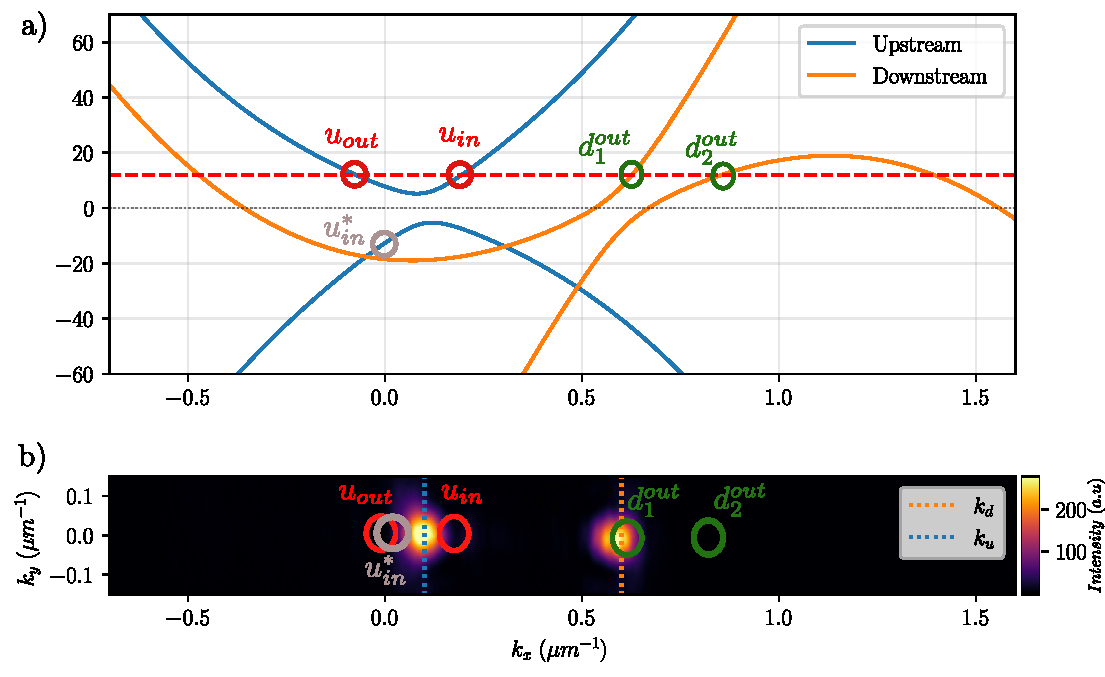
\includegraphics[width=1\textwidth]{chap_stimulated_hawking/fig/bh_k_space.pdf}
    \caption{\textbf{a)} Analytical Bogoliubov dispersion of both regions calculated with the parameters of the fluid of \autoref{fig:typical_dens_2D)} \textbf{a)}. To reflects what happen in practice, the two dispersion are plotted in the same graph as a function of the wavevector in the laboratory frame $k$. The upstream dispersion
    is centered at $k_u$ while the downstream one is centered at $k_d$. The red dashed line corresponds to the energy of the injected mode. The wavevectors of the reflected-transmitted is obtained 
    at the intersections of this line with the Bogoliubov branches and reported in the momentum space \textbf{b)}.The red (resp. green) circle represent the expected location 
    of the upstream (resp. downstream) modes. Finally, the grey circle represent the conjugated of the injected signal resulting from four wave mixing. \textbf{b)} Momentum space of \autoref{fig:typical_dens_2D)} \textbf{a)} : the two bright spots correspond to the two region of the fluid with wavevectors $k_u$ and $k_d$. The colored circle
    are reported from \textbf{a)}.}
    \label{fig:bh_k_space}
\end{figure}

\begin{itemize}
    \item \textbf{Enhancement of the signal}: As discussed in the previous chapter, this can be accomplished by increasing the steepness of the horizon.
    \item \textbf{Suppression of the pump background}: The photonic nature of the system allows us to exploit two key properties of light—polarization and coherence. Polarization filtering can be applied in the detection path, while coherence enables the use of interferometric techniques, as will be detailed in the following section.
\end{itemize}

\textbf{Electronic filtering.} One possible strategy to suppress the pump background is inspired by the method used to measure the excitation spectrum in the previous chapter. By modulating the probe beam intensity at a frequency \(\omega_{\text{mod}}\) accessible in the electronic domain, the signal can later be demodulated, isolating the component arising from the probe-induced excitation. However, in the current context, what previously served as an advantage becomes a limitation. Indeed, the four-wave mixing signals also carry the modulation, thus failing to resolve the overlap problem discussed above. To overcome this, we turn to the optical domain, specifically to interference-based detection schemes.

\subsection{Interferometric Reconstruction of the Fluctuation Field}

The principle of the measurement is to employ the same off-axis interferometric technique previously used to characterize the mean field in both phase and amplitude. The only 
difference is that we aim at using it to reconstruct the fluctuations field. T
